\documentclass[12pt]{article}
\usepackage[margin=1in]{geometry}
\usepackage{fancyvrb}
\usepackage{multicol}
\usepackage{hyperref}
\usepackage{amsmath}
\usepackage{amsfonts}

\usepackage[listings]{tcolorbox}

\definecolor{codegreen}{rgb}{0,0.6,0}
\definecolor{codegray}{rgb}{0.5,0.5,0.5}
\definecolor{codepurple}{rgb}{0.58,0,0.82}
\definecolor{backcolour}{rgb}{0.95,0.95,0.92}

\lstdefinestyle{mystyle}{
    language=Python,
    backgroundcolor=\color{backcolour},   
    commentstyle=\color{codegreen},
    keywordstyle=\color{magenta},
    numberstyle=\tiny\color{codegray},
    stringstyle=\color{codepurple},
    basicstyle=\ttfamily\footnotesize,
    breakatwhitespace=false,         
    breaklines=true,                 
    captionpos=b,                    
    keepspaces=true,                 
    numbers=left,                    
    numbersep=5pt,                  
    showspaces=false,                
    showstringspaces=false,
    showtabs=false,                  
    tabsize=2,
    escapechar=|,
    frame=single
}

\lstset{style=mystyle}

\newcommand{\showfig}[2]{
\noindent\includegraphics[width=\textwidth]{#1}
\centerline{#1}
}

\begin{document}
\sloppy
\centerline{\Large CSCI 111, Lab 11}
\centerline{\large 3d height field visualizer}


\begin{description}
\item[Due date:] Midnight, Tuesday, December 6, on Canvas.
No late work accepted.  

\item[File names:]  Names of files, functions, and variables, 
when specified,
must be EXACTLY as specified.  This includes simple mistakes such
as capitalization.

\item[Individual work:]  All work must be your own.  Do not share
code with anyone other than the instructor and teaching assistants.
This includes looking over shoulders at screens with the code open.
You may discuss ideas, algorithms, approaches, {\em etc.} with
other students but NEVER actual code.

\item[3d vector type:]  You will need your solution to Lab 10,
the vector module, for this assignment.  Add the following method
to the class.  It returns the cross product of two vectors,
a vector perpendicular to both.

\begin{lstlisting}
    def cross(self, other):
        a1, a2, a3 = self.x, self.y, self.z
        b1, b2, b3 = other.x, other.y, other.z
        s1 = a2*b3 - a3*b2
        s2 = a3*b1 - a1*b3
        s3 = a1*b2 - a2*b1
        return V(s1,s2,s3)
\end{lstlisting}
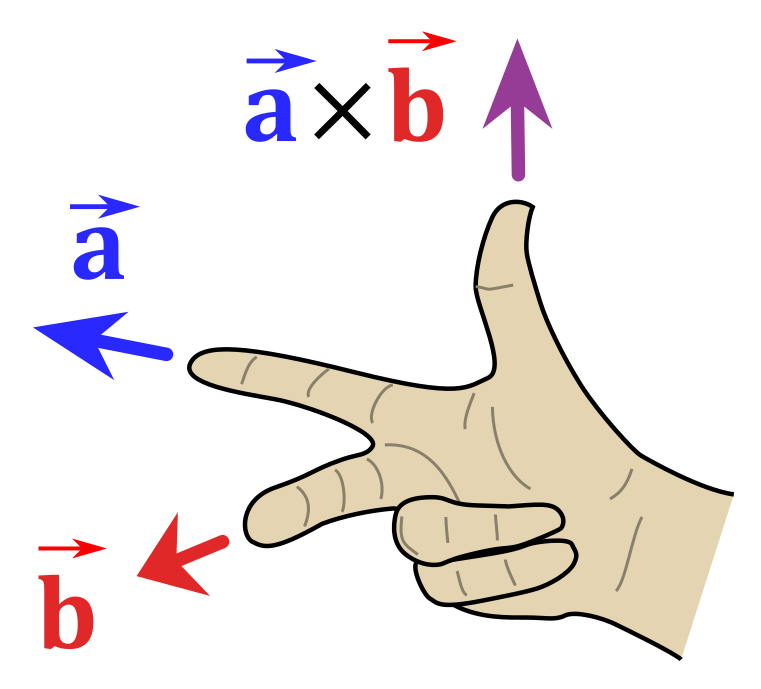
\includegraphics[scale=0.2]{crossproduct}

If you didn't finish this project you can use my implementation,
available on the lab website.

\item[The program]  In the folder \lstinline{poly3d} on the
lab website you can find a skeleton of this program.  The main
program, \lstinline{poly3d.py} is complete, as well as the 
\lstinline{vector.py}, \lstinline{functions.py}, \lstinline{gradient.py}
 and \lstinline{polygon.py}
modules.

You will only have to complete the \lstinline{parametricsurface.py} module.

\item[Step 1, heightfield:]  
Start with implementing \lstinline{makeHeightfield}.  
This should create an empty dictionary.  Loop over
i and j in range(n), and lerp i and j into the xrange 
and yrange, getting x and y in world space.
Applying the function to x and y gives z in world
space.  Store (x,y,z) in self.heightfield[i,j]

Test this with a simple function, for example x+y,
in the range 1..10 with n=10.  Print out the heightfield
so you can see it's working.

\item[Step 2, project points:] 
Now project these points using the eye vector.
The method to make an orthonormal frame around 
the eye is part of the \lstinline{Poly3d} object.

Create a forward, up, right frame around the eye,
and then take the dot product of the 3d point in the heightframe
with the right and up vectors to get the two dimensional
x,y values in the camera frame.  For each [i,j]
store the x,y tuple in \lstinline{self.points[i,j]}.

Also calculate the distance from the point to the eye.
This is just the length of the vector from the point to the eye.
Store these in \lstinline{self.distance[i,j]}

Also, since we're calculating every x,y value for every point,
we can also remember the minima and maxima for both
x and y.  Save these, as well, in \lstinline{self.minx} etc.

Test this on some simple heightframes with some simple
eyes.  For example, what would you expect if the eye 
is V(1,0,0)?  What about V(0,1,0)?

\item[Step 3, make polygons:]
Now make polygons out of the projected points.
For each point with i,j in range(n-1), use the points
at [i,j], [i+1,j], [i+1,j+1], [i,j+1] to make a polygon.
Use the average of these four distances as the
distance to the polygon.  You can use blue, \lstinline{'#0000ff'}
for the color.

Sort your polygons by distance, farthest first.

The best way to test now is to rerun the \lstinline{poly3d}
module, which will plot all your polygons.  Not good?  Debug!

\item[Step 4, add color:] Go back to where you projected all the
points, in Step  2.  Use the gradient object to find the color
of the point, based on the z value in 3d.  Store these in
\lstinline{self.color[i,j]}  

Now go to the step where we made polygons, and 
add this color to the polygon, instead of blue.

Replot. Colorful?

\item[Step 5, shading:] Go back to where you
found the color using the gradient and the z value.

Find the normal to the surface at [i,j] using the cross
product of the vectors from [i,j] to [i+1,j] and from [i,j] to [i,j+1].
Take the dot product of this vector
and a normalized vector pointing to the light.

You can put the light anywhere you want.  Mine is in
this direction: \lstinline{V(2,-1,4)} .  Remember to normalize
the light vector!

The dot product of the normal and the light gives you the shade value,
but it if's less than 0.25 use 0.25 instead of the value.  

\end{description}



\end{document}
